\subsection{Fixed-Parameter Leave One Patient Out Benchmarks}
Logistic regression achieved the highest pooled AUC (0.874), while random forest achieved the highest accuracy (0.799), sensitivity (0.839), and F1 (0.808) among predictive models (Table~\ref{tab:building-lopo-results}). Logistic regression detected 132 of 161 positive records and correctly classified 118 of 158 controls; random forest detected 135 positive records and correctly classified 120 controls. Stacking had the highest specificity (0.772).

\begin{table*}[t]
\centering
\footnotesize
\caption{Fixed-parameter Leave One Patient Out evaluation on 319 held-out predictions per model at threshold 0.5.}
\label{tab:building-lopo-results}
\begin{tabular}{@{}lrrrrrr@{}}
\toprule
Model & Accuracy & ROC--AUC & Sensitivity & Specificity & F1 & FNR \\
\midrule
Logistic regression & 0.784 & \textbf{0.874} & 0.820 & 0.747 & 0.793 & 0.180 \\
Random forest & \textbf{0.799} & 0.857 & \textbf{0.839} & 0.759 & \textbf{0.808} & \textbf{0.161} \\
XGBoost & 0.762 & 0.835 & 0.807 & 0.715 & 0.774 & 0.193 \\
LightGBM & 0.787 & 0.851 & 0.832 & 0.741 & 0.798 & 0.168 \\
Stacking & 0.787 & 0.865 & 0.801 & \textbf{0.772} & 0.791 & 0.199 \\
\midrule
Training-prior dummy & 0.505 & 0.000 & 1.000 & 0.000 & 0.671 & 0.000 \\
\bottomrule
\end{tabular}
\end{table*}
The training-prior dummy's pooled AUC of 0.000 is a leave-one-out artefact: excluding a positive record lowers its training prevalence, while excluding a negative record raises it. Its pooled probabilities therefore rank the classes inversely, even though every thresholded prediction is positive. The value is not evidence of useful discrimination.

The single LOPO run compares fixed pipelines using the same excluded records; it does not estimate between-seed variability or the performance of a nested model-selection procedure.

\subsection{Optuna-Tuned Leave One Patient Out Benchmarks}
All five predictive families completed 319 outer folds with 20 Optuna trials and three stratified inner folds per outer training set. The source-data signature, feature count, seed, threshold, and dependency versions were identical across tuned runs. The first five rows of Table~\ref{tab:tuned-lopo-results} are these historical fixed-RFE20 runs; the final row is updated stacking with a searched feature count. All scores evaluate pooled held-out predictions, not inner validation scores.

\begin{table*}[t]
\centering\footnotesize
\setlength{\tabcolsep}{4pt}
\caption{Completed Optuna LOPO test results: 319 held-out predictions per configuration, seed 42, twenty trials, three inner folds and threshold 0.5. The first five rows use fixed RFE20; updated stacking searches k in 10/20/30/38 and tunes XGBoost/LightGBM/ridge bases with a fixed logistic meta learner. Bold marks the best observed value (lower for FNR/FN). Different search designs limit causal comparisons.}
\label{tab:tuned-lopo-results}
\begin{tabular}{@{}lrrrrrrrr@{}}
\toprule
Model/configuration & Accuracy & ROC--AUC & Precision & Sensitivity & Specificity & F1 & FNR & FN \\
\midrule
Logistic regression & 0.7868 & 0.8680 & 0.7688 & 0.8261 & 0.7468 & 0.7964 & 0.1739 & 28 \\
Random forest & 0.7743 & 0.8421 & 0.7602 & 0.8075 & 0.7405 & 0.7831 & 0.1925 & 31 \\
XGBoost & 0.7837 & 0.8509 & 0.7644 & 0.8261 & 0.7405 & 0.7940 & 0.1739 & 28 \\
LightGBM & 0.7868 & 0.8395 & 0.7751 & 0.8137 & 0.7595 & 0.7939 & 0.1863 & 30 \\
Stacking (historical, meta-tuned) & 0.7837 & 0.8617 & 0.7738 & 0.8075 & 0.7595 & 0.7903 & 0.1925 & 31 \\
\midrule
Stacking (updated, base-tuned) & \textbf{0.8056} & \textbf{0.8762} & \textbf{0.7895} & \textbf{0.8385} & \textbf{0.7722} & \textbf{0.8133} & \textbf{0.1615} & \textbf{26} \\
\bottomrule
\end{tabular}
\end{table*}

Within the historical fixed-RFE20 comparison, tuned logistic regression retained the highest AUC (0.868) and F1 (0.796), with accuracy 0.787 and sensitivity 0.826. It detected 133 of 161 cases and correctly classified 118 of 158 controls. XGBoost matched its sensitivity and false-negative count (28), but had lower AUC (0.851) and one additional false positive (41 versus 40). LightGBM matched the highest accuracy (0.787), while LightGBM and stacking shared the highest specificity (0.759). Random forest achieved AUC 0.842 and sensitivity 0.807. Stacking did not exceed logistic regression in discrimination or sensitivity; only its logistic meta-learner was tuned, with fixed base-model settings.

\subsection{Updated Base-Tuned Stacking with Joint Feature Selection}
The completed search-version-3 stacking run evaluated all 319 outer exclusions using seed 42, twenty Optuna trials per exclusion and three stratified inner validation folds. Unlike the historical meta-only search, this run jointly tuned XGBoost, LightGBM and ridge base learners and the RFE feature count; the standardised logistic meta-learner remained fixed at $C=1$. Table~\ref{tab:tuned-lopo-results} reports metrics recomputed from the saved outer predictions, not averages of inner validation scores.



The updated stack correctly classified 257 of 319 records: TN=122, FP=36, FN=26 and TP=135. Its AUC increased descriptively by 0.0145 and five fewer positive records were missed relative to the historical tuned stack. Across completed tuned experiments, this configuration has the highest observed AUC, accuracy, sensitivity, specificity and F1. These rankings are descriptive: the standalone candidates have not been rerun with the new feature-count search, and no significance or independent replication is established.

Optuna selected 10 features in one outer fold, 20 in 45 folds, 30 in 34 folds and all 38 in 239 folds. This favours the full input set in most exclusions and does not support a claim that a reduced twenty-field subset is optimal for the updated stack. The arithmetic mean selected-trial inner-validation AUC was 0.8747 across exclusions; it is a tuning diagnostic, not the outer test AUC, and its heavily overlapping validation sets are not independent replications.

The source evidence is \path{results/stacking_v3}: configuration, 319 prediction rows, 319 outer checkpoints, 6,380 completed Optuna trials and \path{CV_Metrics/stacking.csv}. The latter retains the selected trial's three-fold mean, sample standard deviation and individual-fold accuracy, AUC, precision, recall, specificity and sensitivity, plus selected feature count. Recall and sensitivity denote the same positive-class quantity. The new stack changes base composition, tuning scope, feature-count search and sampler-seed scheduling together; the observed improvement cannot be attributed to one change alone. SHAP/LIME figures below still explain the historical tuned logistic models and have not been regenerated for the new stack.

\subsection{Historical Changes Relative to Fixed Configurations}
XGBoost showed the largest positive change relative to its historical fixed benchmark: AUC increased from 0.835 to 0.851, accuracy from 0.762 to 0.784, and sensitivity from 0.807 to 0.826; false negatives decreased from 31 to 28. Logistic regression's AUC decreased from 0.874 to 0.868, although accuracy increased slightly and one fewer positive record was missed. Random forest's AUC decreased from 0.857 to 0.842, with five additional false negatives (26 to 31). LightGBM's accuracy was unchanged, but AUC decreased from 0.851 to 0.840 and false negatives increased from 27 to 30. Stacking's AUC decreased from 0.865 to 0.862; one fewer false negative was offset by two additional false positives.

These differences are descriptive rather than evidence that tuning alone caused the changes. The historical fixed run used scikit-learn 1.7.1, whereas the tuned runs used 1.9.1; NumPy and pandas versions also differed. Although the cohort and outer record exclusions were shared, a controlled estimate of tuning's effect requires refitting the fixed configurations in the tuned environment. No significance test or confidence interval was calculated. Optimising inner-fold AUC did not consistently improve outer discrimination or classification at threshold 0.5, and the search budget does not establish globally optimal parameters.


\subsection{Confusion Matrices and Average Classification Error}
Figure~\ref{fig:experimental-confusion} reproduces the saved fixed-parameter Experimental LOPO ROC/confusion-matrix figure and adds a descriptive mean confusion matrix across the five predictive families in Table~\ref{tab:building-lopo-results}, excluding the dummy. Mean counts were 118.0 true negatives, 40.0 false positives, 29.0 false negatives, and 132.0 true positives. The mean classification error was $(40+29)/319=21.6\%$, with mean false-negative rate $29/161=18.0\%$. This averages model-specific counts on the same 319 held-out records; it is not an ensemble confusion matrix, an average across seeds, or a set of independent replications. Tuned logistic regression, which is explained in the XAI results, instead had 118 true negatives, 40 false positives, 28 false negatives, and 133 true positives.

\begin{figure*}[t]
\centering
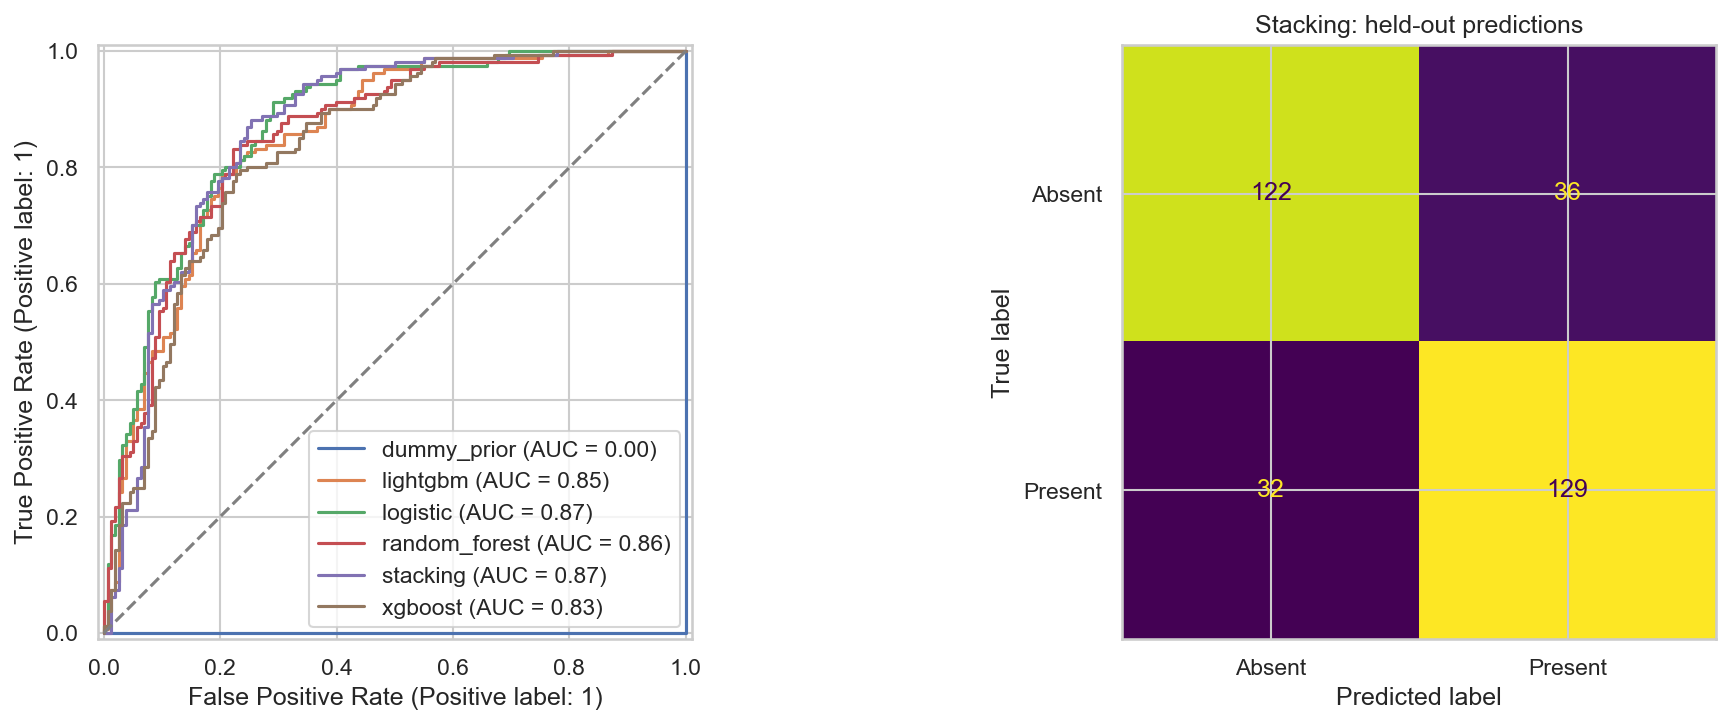
\includegraphics[width=0.97\linewidth]{figures/evaluation/experimental_lopo_roc_confusion.png}
\par\medskip
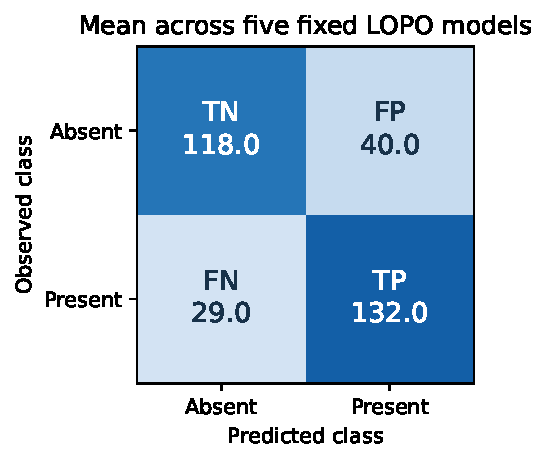
\includegraphics[width=0.43\linewidth]{figures/evaluation/average_fixed_lopo_confusion.pdf}
\caption{Fixed-parameter Experimental LOPO results at threshold 0.5. Top: existing ROC curves and the stacking confusion matrix (TN=122, FP=36, FN=32, TP=129). Bottom: arithmetic mean counts across logistic regression, random forest, XGBoost, LightGBM, and stacking, each evaluated on the same 319 records. The mean summarises model errors and does not represent predictions from a single classifier.}
\label{fig:experimental-confusion}
\end{figure*}

\subsection{Recurring Classification Errors in Fixed Models}
Source record 117 was a false negative in four of the five predictive LOPO models. Records 291 and 316 were false positives in all five. These retrospectively identified examples indicate disagreement between observed labels and predictions across model families, without establishing clinical causes or labelling errors. They support inspecting common failure cases in addition to aggregate discrimination and classification metrics.

\subsection{SHAP and LIME Explanations of Tuned Logistic Regression}
All XAI results in this subsection explain the Optuna-tuned logistic regression pipeline, using a separately fitted outer-fold model for each held-out record. The fixed logistic regression, random forest, XGBoost, LightGBM, and stacking benchmarks were not the models explained in these figures. Figure~\ref{fig:xai-global} summarises the 20 sampled held-out explanations from the tuned logistic models. The largest mean absolute SHAP contributions were associated with the source fields \texttt{bm} (0.208), CRP (0.173), extracellular-fluid/total-body-water ratio (0.071), vitamin D (0.068), weight (0.065), and extracellular water (0.056). The ordering describes this small sample and the fold-specific models, rather than a population-level ranking. Higher recorded CRP values generally contributed towards the absent class within these fitted models; this association does not imply a protective biological effect.

\begin{figure}[tbp]
\centering
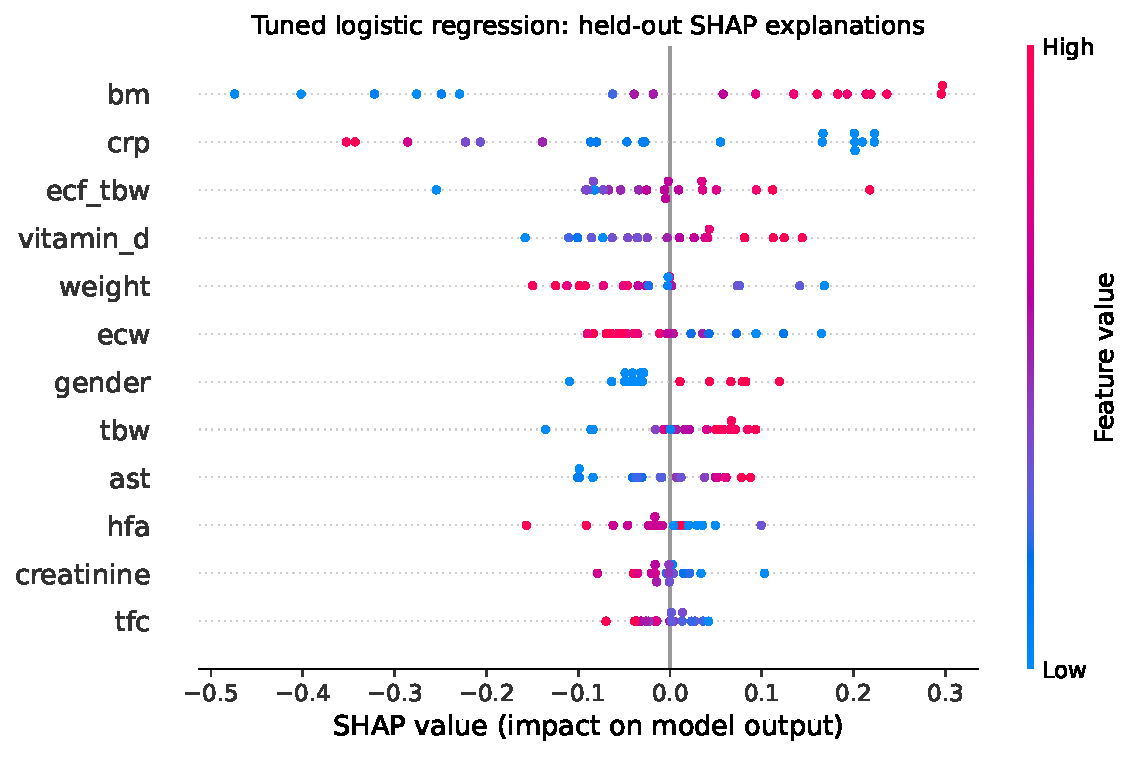
\includegraphics[width=0.88\linewidth]{figures/xai/global_shap.pdf}
\caption{Kernel SHAP summary for 20 sampled excluded records from tuned logistic Leave One Patient Out models. Each point uses its own outer-fold model and training-only background. Positive values increase the predicted probability of gallstones; negative values decrease it. Colour indicates the recorded feature value, and source-field labels follow the dataset schema. Features are ordered by sampled mean absolute contribution.}
\label{fig:xai-global}
\end{figure}

Figure~\ref{fig:xai-errors} compares SHAP and LIME for two confident errors. Source record 156 was a false negative with predicted probability 0.038; its largest displayed negative SHAP contributions included fluid ratio, \texttt{bm}, and vitamin D. Source record 178 was a false positive with predicted probability 0.995. These examples illustrate how multiple contributions can support an incorrect prediction despite aggregate discrimination. SHAP baselines were 0.443 and 0.413, respectively, and reconstruction from all feature contributions matched the saved probabilities. Only the eight largest contributions are displayed locally.

LIME surrogate $R^2$ was 0.423 for the false negative and 0.230 for the false positive, indicating limited local fidelity. For record 156, the surrogate prediction (0.160) also differed from the classifier probability (0.038). LIME condition weights and SHAP probability contributions have different meanings and should not be compared numerically. Agreement in direction is descriptive; correlated measurements and synthetic perturbations can produce unstable or implausible neighbourhoods.

\begin{figure*}[t]
\centering
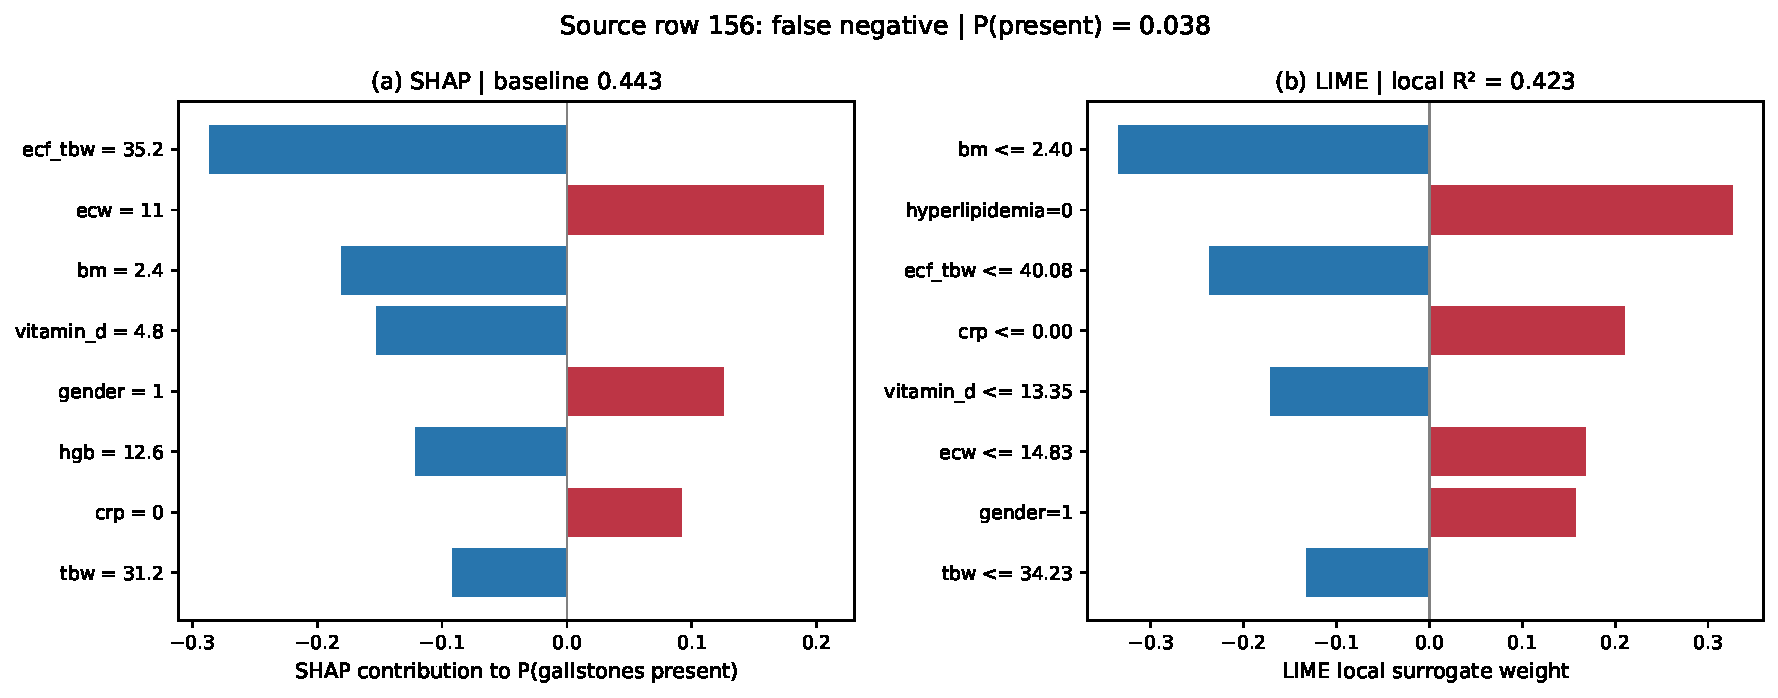
\includegraphics[width=0.88\linewidth]{figures/xai/local_fn.pdf}
\par\medskip
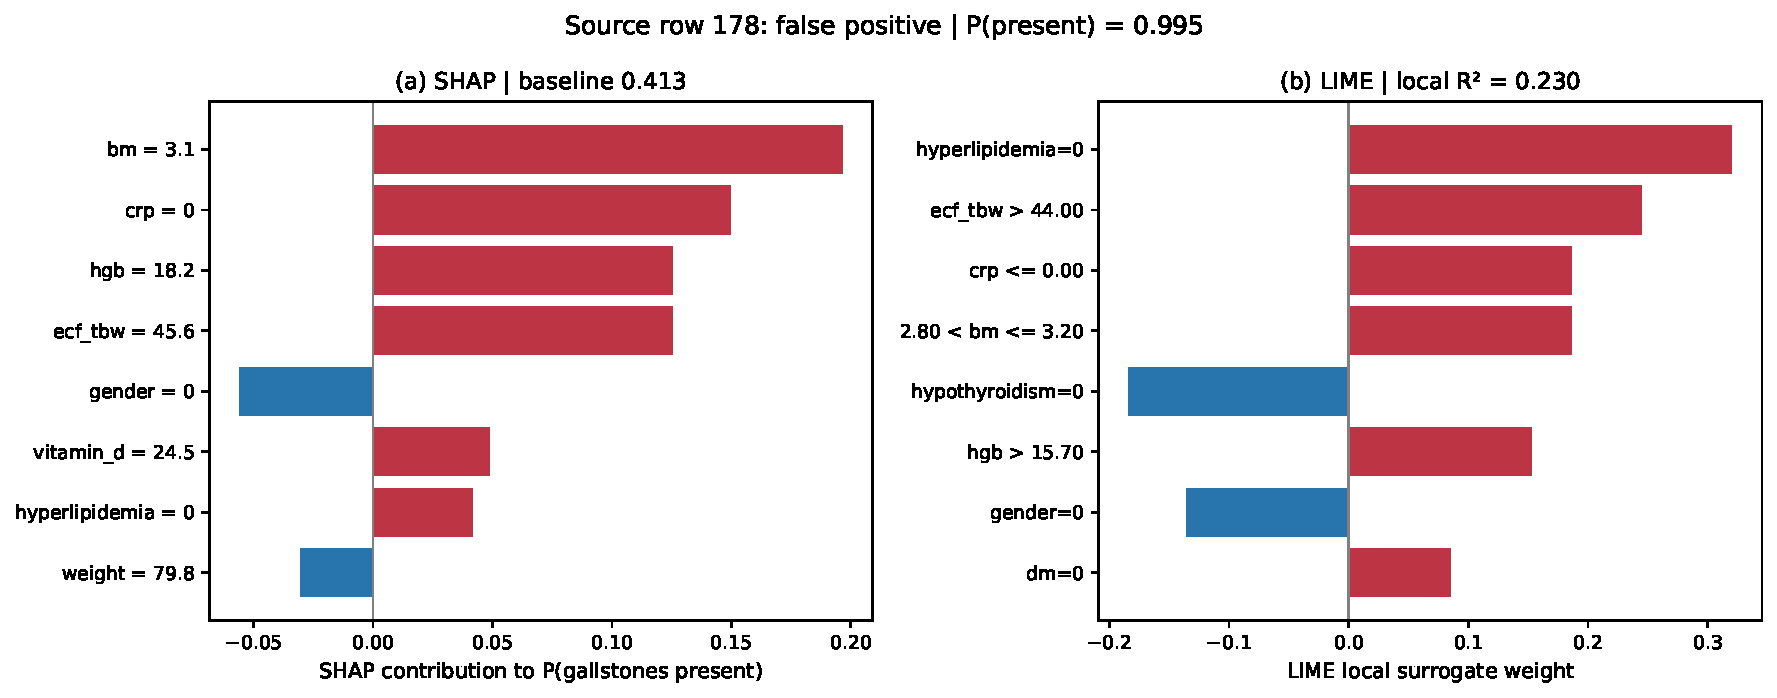
\includegraphics[width=0.88\linewidth]{figures/xai/local_fp.pdf}
\caption{Local explanations of a retrospectively selected false negative (source row 156, top) and false positive (source row 178, bottom) from tuned logistic Leave One Patient Out evaluation. Left: the eight largest absolute SHAP contributions, labelled with recorded input values. Right: LIME condition weights and local surrogate fidelity. Red pushes towards gallstones present; blue pushes towards absent. Each excluded record was omitted from fitting, tuning, and explainer background construction. These selected examples do not estimate error prevalence.}
\label{fig:xai-errors}
\end{figure*}

